\section{Base Legal}\label{sec:base_legal}
Aqui ser� a parte reservada para relatar a sustenta��o legal do pesquisa, tendo como base norteadora o PCN e o PCN+. Tamb�m comentarei aqui a import�ncia do tema para as avalia��es de larga escala, como o Exame Nacional do Ensino M�dio (ENEM).

%\begin{table}
%\caption{Exemplo de uma Tabela}
%\label{minhatab}

%\center
%\begin{tabular}{cccc}
%  % after \\: \hline or \cline{col1-col2} \cline{col3-col4} ...
%  \hline
%	Par�metro & Unidade & Valor da simula��o & Valor experimental   \\
%	\hline
%  Comprimento, $\alpha$ & $m$ &  $8,23$  & $8,54$ \\
%  Altura, $\beta$ & $m$     &  $29,1$ & $28,3$\\
%	Velocidade, $v$ & $m/s$  &  $60,2$ & $67,3$\\
%	\hline
%\end{tabular}
%\end{table}


%\begin{figura}[h]
%\centering
%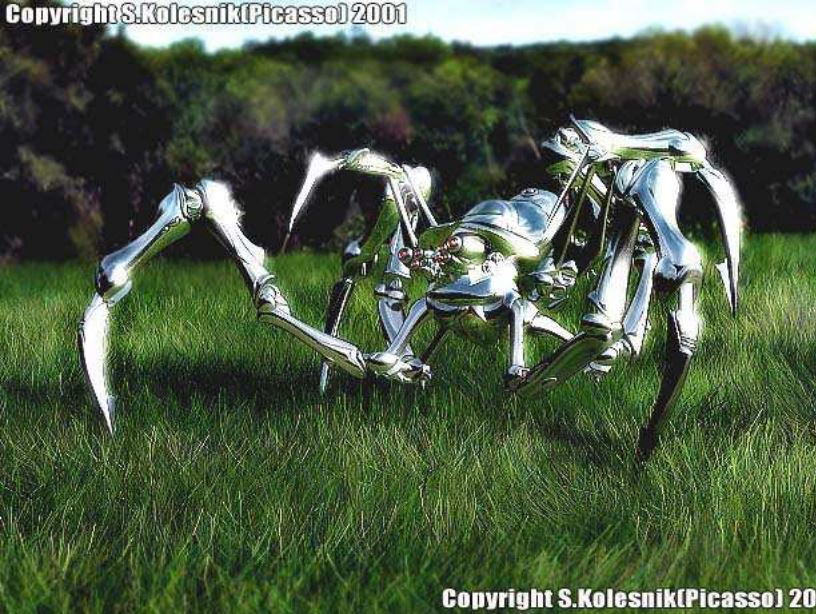
\includegraphics[width=0.5\textwidth]{Fundamentacao_Teorica/spiderrobot}
%\caption{Cupim cibern�tico.} \label{FDIII}
%\end{figura}

%\begin{figura}[h]
%	\centering
%	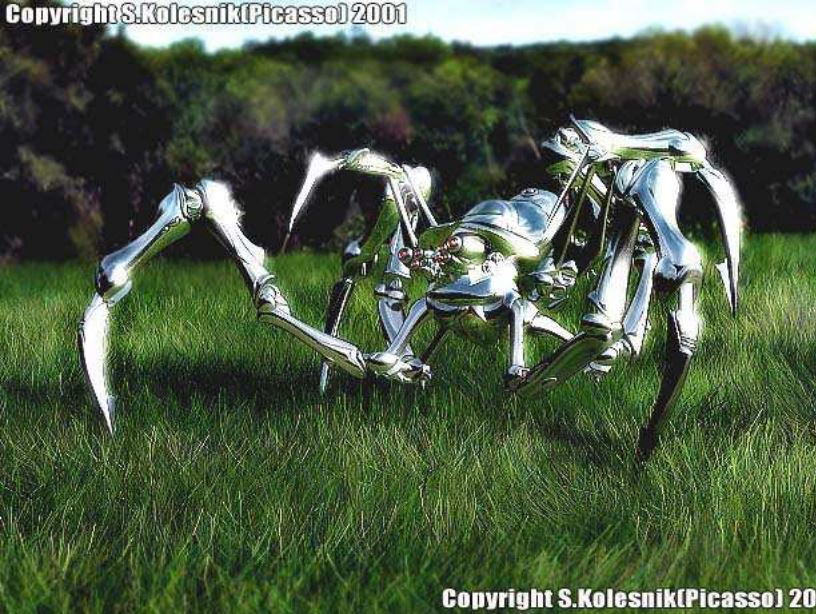
\includegraphics[width=0.75\textwidth]{Fundamentacao_Teorica/spiderrobot}
%	\caption{Cupim cibern�tico.} \label{FDIII}
%\end{figura}

%\begin{tabela}[h]
%	\centering
%	%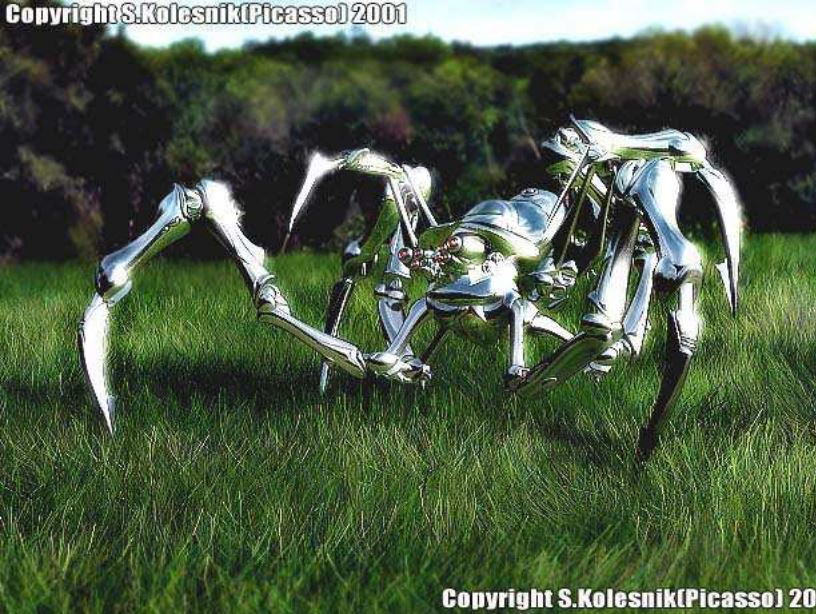
\includegraphics[width=0.75\textwidth]{Fundamentacao_Teorica/spiderrobot}
%	\caption{Cupim cibern�tico.} \label{FDIII}
%\end{tabela}

%\begin{quadro}[h]
%	\centering
%	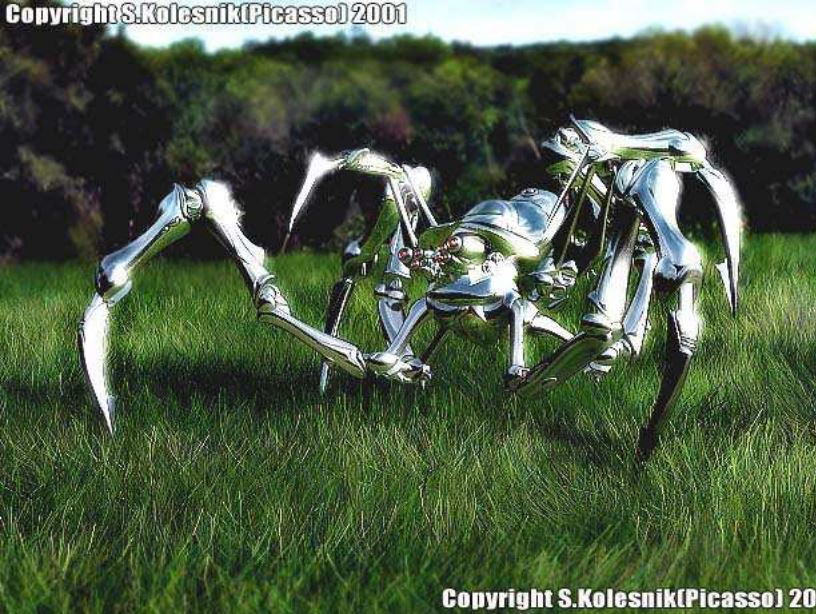
\includegraphics[width=0.75\textwidth]{Fundamentacao_Teorica/spiderrobot}
%	\caption{Cupim cibern�tico.} \label{FDIII}
%\end{quadro}


%\begin{equation} \label{eq:lagr1}
%\frac{d}{dt}(\frac{\partial L}{\partial \dot{q}})-\frac{\partial L}{\partial q}=\tau^{T}.
%\end{equation}


\section{Referenciais Te�ricos}\label{sec:referenciais_te�ricos}
Aqui ser� a se��o reservada para destacar os referenciais te�ricas que ir�o nortear a pesquisa: David Ausubel e Marc Prensky.
\subsection{David Ausubel - Aprendizagem Significativa}\label{subsec:ausubel}
Aqui comentarei sobre a import�ncia da teoria da aprendizagem significativa para a minha pesquisa, pois toda a minha sequ�ncia did�tica � permeada por esta teoria.
\subsection{Marc Prensky - Aprendizagem Baseada em Jogos Digitais}\label{subsec:prensky}
J� aqui, ser� uma abordagem mais espec�fica da aprendizagem baseada em jogos digitais.

\section{Revis�o de Trabalhos Relacionados com o Tema}\label{sec:revis�o_de_trabalhos}
Aqui nesta se��o, farei uma breve revis�o liter�ria da produ��o digital relacionada � F�sica Moderna no Ensino M�dio. Farei uma levantamento da produ��o de jogos, simula��es e aplicativos relacionados ao tema. 

\subsection{F�sica de Part�culas no Ensino M�dio}

\subsection{Jogos Digitais}

